% ============================================================
% Question Bank: ch01-06 Applying Proportional Reasoning (Modified — OK)
% Topic Title: Applying Proportional Reasoning (OAS-M estimation emphasis)
% CCSS: 7.RP.A.2, 7.RP.A.3 (Modified)
% Questions: 30 (18 MC + 7 SA + 5 Graphical)
% ============================================================

% --- Multiple Choice Questions (18) ---

\begin{practiceQuestion}{m-1-6-q01}{mc}
\begin{questionText}
A car travels $180$ miles on $6$ gallons of gas. Which is the best estimate for the distance it can travel on $9$ gallons?
\end{questionText}
\choiceA{About $200$ miles}
\choiceB{About $270$ miles}
\choiceC{About $360$ miles}
\choiceD{About $186$ miles}
\correctAnswer{B}
\explanation{Estimate: $180 \div 6 = 30$ mpg. $30 \times 9 = 270$ miles.}
\end{practiceQuestion}

\begin{practiceQuestion}{m-1-6-q02}{mc}
\begin{questionText}
You buy $3$ notebooks for $\$7.50$. Which is the best way to estimate the cost of $7$ notebooks?
\end{questionText}
\choiceA{Round $\$7.50 \div 3 \approx \$2$, then $\$2 \times 7 = \$14$}
\choiceB{Round $\$7.50 \div 3 \approx \$2.50$, then $\$2.50 \times 7 = \$17.50$}
\choiceC{Multiply $\$7.50 \times 7 = \$52.50$}
\choiceD{Add $\$7.50 + 7 = \$14.50$}
\correctAnswer{B}
\explanation{First find the unit rate: $\$7.50 \div 3 = \$2.50$ per notebook. Then multiply: $\$2.50 \times 7 = \$17.50$.}
\end{practiceQuestion}

\begin{practiceQuestion}{m-1-6-q03}{mc}
\begin{questionText}
A baker uses $4$ cups of flour for $10$ muffins. She needs to make $25$ muffins. She estimates she needs about $10$ cups of flour. Is her estimate reasonable?
\end{questionText}
\choiceA{Yes — $25$ is $2.5$ times $10$, and $2.5 \times 4 = 10$}
\choiceB{No — she needs $6.25$ cups, not $10$}
\choiceC{No — she needs $100$ cups}
\choiceD{Yes — but only if she rounds up}
\correctAnswer{A}
\explanation{$25$ muffins is $2.5$ times $10$ muffins, so she needs $2.5 \times 4 = 10$ cups. The estimate is correct.}
\end{practiceQuestion}

\begin{practiceQuestion}{m-1-6-q04}{mc}
\begin{questionText}
A printer prints $90$ pages in $6$ minutes. Which proportion could you use to find how long it takes to print $300$ pages?
\end{questionText}
\choiceA{$\dfrac{90}{6} = \dfrac{300}{t}$}
\choiceB{$\dfrac{90}{6} = \dfrac{t}{300}$}
\choiceC{$\dfrac{6}{300} = \dfrac{90}{t}$}
\choiceD{$\dfrac{90}{300} = \dfrac{6}{t}$}
\correctAnswer{A}
\explanation{The ratio of pages to minutes is $\frac{90}{6}$. Set it equal to $\frac{300}{t}$ and solve: $t = 20$ minutes.}
\end{practiceQuestion}

\begin{practiceQuestion}{m-1-6-q05}{mc}
\begin{questionText}
Brand~A juice costs $\$3.60$ for $6$ bottles. Brand~B costs $\$5.00$ for $8$ bottles. Which is the better deal?
\end{questionText}
\choiceA{Brand A — $\$0.50$ per bottle}
\choiceB{Brand A — $\$0.60$ per bottle}
\choiceC{Brand B — $\$0.625$ per bottle}
\choiceD{Brand B — $\$0.50$ per bottle}
\correctAnswer{B}
\explanation{Brand A: $3.60 \div 6 = \$0.60$/bottle. Brand B: $5.00 \div 8 = \$0.625$/bottle. Brand A is cheaper per bottle, at $\$0.60$.}
\end{practiceQuestion}

\begin{practiceQuestion}{m-1-6-q06}{mc}
\begin{questionText}
A recipe for $6$ servings uses $\frac{3}{4}$ cup of sugar. You want $15$ servings. A student estimates she needs about $2$ cups. Is this reasonable?
\end{questionText}
\choiceA{Yes — $15$ is $2.5 \times 6$, and $2.5 \times \frac{3}{4} \approx 2$}
\choiceB{No — she needs exactly $\frac{15}{4}$ cups}
\choiceC{No — she only needs $1$ cup}
\choiceD{Yes — but only if she doubles the recipe}
\correctAnswer{A}
\explanation{Scale factor: $15 \div 6 = 2.5$. Sugar: $2.5 \times \frac{3}{4} = \frac{15}{8} = 1.875$ cups, which rounds to about $2$ cups. Reasonable.}
\end{practiceQuestion}

\begin{practiceQuestion}{m-1-6-q07}{mc}
\begin{questionText}
On a map, $2$ cm represents $16$ km. A road measures $7$ cm. What is the actual distance?
\end{questionText}
\choiceA{$48$ km}
\choiceB{$56$ km}
\choiceC{$64$ km}
\choiceD{$32$ km}
\correctAnswer{B}
\explanation{$1$ cm $= 16 \div 2 = 8$ km. So $7$ cm $= 7 \times 8 = 56$ km.}
\end{practiceQuestion}

\begin{practiceQuestion}{m-1-6-q08}{mc}
\begin{questionText}
A student solved: ``$4$ shirts cost $\$34$. How much for $10$ shirts?'' and got $\$340$. What is the most likely error?
\end{questionText}
\choiceA{She multiplied $\$34 \times 10$ instead of finding the unit rate first}
\choiceB{She divided $\$34$ by $10$}
\choiceC{She added $\$34 + 10$}
\choiceD{She subtracted $\$34 - 10$}
\correctAnswer{A}
\explanation{$\$340$ is $\$34 \times 10$. She should have found the unit rate ($\$8.50$/shirt) first, then multiplied by $10$ to get $\$85$.}
\end{practiceQuestion}

\begin{practiceQuestion}{m-1-6-q09}{mc}
\begin{questionText}
A car uses $8$ gallons of gas to travel $240$ miles. Estimate the gas needed for $500$ miles.
\end{questionText}
\choiceA{About $12$ gallons}
\choiceB{About $15$ gallons}
\choiceC{About $17$ gallons}
\choiceD{About $20$ gallons}
\correctAnswer{C}
\explanation{Estimate: $240 \div 8 = 30$ mpg. $500 \div 30 \approx 16.7$ gallons, which is about $17$ gallons.}
\end{practiceQuestion}

\begin{practiceQuestion}{m-1-6-q10}{mc}
\begin{questionText}
Which strategy finds the answer to ``$3$ kg of apples cost $\$5.25$. How much for $8$ kg?'' using a proportion?
\end{questionText}
\choiceA{$\dfrac{3}{5.25} = \dfrac{8}{x}$ and cross-multiply}
\choiceB{$\dfrac{3}{8} = \dfrac{5.25}{x}$ and cross-multiply}
\choiceC{$5.25 \times 8 = x$}
\choiceD{$3 \times 8 \div 5.25 = x$}
\correctAnswer{A}
\explanation{Set up $\frac{3}{5.25} = \frac{8}{x}$. Cross-multiply: $3x = 42$, so $x = \$14$.}
\end{practiceQuestion}

\begin{practiceQuestion}{m-1-6-q11}{mc}
\begin{questionText}
A runner covers $5$ miles in $40$ minutes. At the same pace, how long will $8$ miles take?
\end{questionText}
\choiceA{$48$ minutes}
\choiceB{$56$ minutes}
\choiceC{$64$ minutes}
\choiceD{$72$ minutes}
\correctAnswer{C}
\explanation{Rate: $40 \div 5 = 8$ min/mile. For $8$ miles: $8 \times 8 = 64$ minutes.}
\end{practiceQuestion}

\begin{practiceQuestion}{m-1-6-q12}{mc}
\begin{questionText}
A paint-mixing ratio is $3$ parts blue to $5$ parts white. If you use $12$ parts blue, how many parts white do you need?
\end{questionText}
\choiceA{$15$}
\choiceB{$20$}
\choiceC{$8$}
\choiceD{$25$}
\correctAnswer{B}
\explanation{Scale factor: $12 \div 3 = 4$. White: $5 \times 4 = 20$ parts.}
\end{practiceQuestion}

\begin{practiceQuestion}{m-1-6-q13}{mc}
\begin{questionText}
A train travels $350$ miles in $5$ hours. Using the equation $y = kx$, what is $k$?
\end{questionText}
\choiceA{$k = 5$}
\choiceB{$k = 70$}
\choiceC{$k = 350$}
\choiceD{$k = 1{,}750$}
\correctAnswer{B}
\explanation{$k$ is the unit rate: $350 \div 5 = 70$ miles per hour. So $y = 70x$.}
\end{practiceQuestion}

\begin{practiceQuestion}{m-1-6-q14}{mc}
\begin{questionText}
A student estimates that $7$ pizzas for a party of $21$ people is enough if each person eats $\frac{1}{3}$ of a pizza. Is the estimate reasonable?
\end{questionText}
\choiceA{Yes — $21 \times \frac{1}{3} = 7$}
\choiceB{No — $21 \times \frac{1}{3} = 63$}
\choiceC{No — you need $21$ pizzas}
\choiceD{Yes — but only if the pizzas are large}
\correctAnswer{A}
\explanation{$21 \times \frac{1}{3} = 7$ pizzas. The estimate matches exactly.}
\end{practiceQuestion}

\begin{practiceQuestion}{m-1-6-q15}{mc}
\begin{questionText}
Small bag: $\frac{1}{2}$ lb of trail mix for $\$2.80$. Large bag: $1\frac{1}{4}$ lb for $\$6.00$. Which is the better deal?
\end{questionText}
\choiceA{Small — $\$5.60$/lb}
\choiceB{Large — $\$4.80$/lb}
\choiceC{They cost the same per pound}
\choiceD{Large — $\$6.00$/lb}
\correctAnswer{B}
\explanation{Small: $2.80 \div 0.5 = \$5.60$/lb. Large: $6.00 \div 1.25 = \$4.80$/lb. The large bag is cheaper per pound.}
\end{practiceQuestion}

\begin{practiceQuestion}{m-1-6-q16}{mc}
\begin{questionText}
An architect's model uses a scale of $1$ inch $= 4$ feet. A hallway in the model is $3.5$ inches long. What is the actual length?
\end{questionText}
\choiceA{$7$ feet}
\choiceB{$12$ feet}
\choiceC{$14$ feet}
\choiceD{$16$ feet}
\correctAnswer{C}
\explanation{$3.5 \times 4 = 14$ feet.}
\end{practiceQuestion}

\begin{practiceQuestion}{m-1-6-q17}{mc}
\begin{questionText}
A factory produces $450$ widgets in $6$ hours. A manager estimates it can produce about $1{,}000$ widgets in $12$ hours. Is this reasonable?
\end{questionText}
\choiceA{No — it should be exactly $900$}
\choiceB{Yes — doubling the time roughly doubles the output, and $900$ is close to $1{,}000$}
\choiceC{No — it should be $5{,}400$}
\choiceD{Yes — $1{,}000$ is exactly right}
\correctAnswer{A}
\explanation{Unit rate: $450 \div 6 = 75$ per hour. In $12$ hours: $75 \times 12 = 900$. The estimate of $1{,}000$ is too high; the exact answer is $900$.}
\end{practiceQuestion}

\begin{practiceQuestion}{m-1-6-q18}{mc}
\begin{questionText}
A student solved a proportion and got $\$12$ for $20$ gallons of gas. She checks by estimating: gas costs about $\$3$--$\$5$ per gallon. What should she conclude?
\end{questionText}
\choiceA{Her answer is reasonable}
\choiceB{Her answer is too low — $20$ gallons should cost $\$60$--$\$100$}
\choiceC{Her answer is too high}
\choiceD{She cannot check without more information}
\correctAnswer{B}
\explanation{At $\$3$/gal, $20$ gallons costs $\$60$. At $\$5$/gal, it costs $\$100$. $\$12$ is far too low, so she made an error.}
\end{practiceQuestion}

% --- Short Answer Questions (7) ---

\begin{practiceQuestion}{m-1-6-q19}{sa}
\begin{questionText}
A recipe calls for $\frac{2}{3}$ cup of milk for $4$ pancakes. How many cups are needed for $18$ pancakes?
\end{questionText}
\correctAnswer{$3$ cups}
\explanation{Unit rate: $\frac{2}{3} \div 4 = \frac{1}{6}$ cup per pancake. For $18$: $\frac{1}{6} \times 18 = 3$ cups.}
\end{practiceQuestion}

\begin{practiceQuestion}{m-1-6-q20}{sa}
\begin{questionText}
A car travels $275$ miles on $11$ gallons. What is the unit rate in miles per gallon?
\end{questionText}
\correctAnswer{$25$ mpg}
\explanation{$275 \div 11 = 25$ miles per gallon.}
\end{practiceQuestion}

\begin{practiceQuestion}{m-1-6-q21}{sa}
\begin{questionText}
On a map, $5$ cm represents $40$ km. How far apart are two cities that are $12$ cm apart on the map?
\end{questionText}
\correctAnswer{$96$ km}
\explanation{$1$ cm $= 40 \div 5 = 8$ km. $12 \times 8 = 96$ km.}
\end{practiceQuestion}

\begin{practiceQuestion}{m-1-6-q22}{sa}
\begin{questionText}
A machine fills $360$ bottles in $8$ minutes. How many bottles does it fill in $15$ minutes?
\end{questionText}
\correctAnswer{$675$ bottles}
\explanation{Rate: $360 \div 8 = 45$ bottles per minute. $45 \times 15 = 675$ bottles.}
\end{practiceQuestion}

\begin{practiceQuestion}{m-1-6-q23}{sa}
\begin{questionText}
$6$ T-shirts cost $\$52.50$. Estimate the cost of $10$ T-shirts, then find the exact amount.
\end{questionText}
\correctAnswer{$\$87.50$}
\explanation{Estimate: $\$52.50 \div 6 \approx \$9$ per shirt, so $10 \times \$9 \approx \$90$. Exact: $52.50 \div 6 = \$8.75$. $8.75 \times 10 = \$87.50$. Check: $\$87.50$ is close to $\$90$. \checkmark}
\end{practiceQuestion}

\begin{practiceQuestion}{m-1-6-q24}{sa}
\begin{questionText}
Store~A sells $3$ lb of chicken for $\$12.75$. Store~B sells $5$ lb for $\$20.00$. Which store has the lower unit price, and what is it?
\end{questionText}
\correctAnswer{Store B at $\$4.00$/lb}
\explanation{Store A: $12.75 \div 3 = \$4.25$/lb. Store B: $20.00 \div 5 = \$4.00$/lb. Store B is cheaper by $\$0.25$ per pound.}
\end{practiceQuestion}

\begin{practiceQuestion}{m-1-6-q25}{sa}
\begin{questionText}
A bus travels $168$ miles in $3$ hours. Use the equation $y = kx$ to find how far it travels in $7$ hours at the same rate.
\end{questionText}
\correctAnswer{$392$ miles}
\explanation{$k = 168 \div 3 = 56$ mph. $y = 56 \times 7 = 392$ miles.}
\end{practiceQuestion}

% --- Graphical Questions (3 GMC + 2 GSA) ---

\begin{practiceQuestion}{m-1-6-q26}{gmc}
\begin{questionText}
The table shows the cost of bags of oranges. Estimate the cost of $9$ bags.

\begin{center}
\begin{tabular}{|c|c|}
\hline
\textbf{Bags} & \textbf{Cost} \\
\hline
$2$ & $\$5.00$ \\
\hline
$4$ & $\$10.00$ \\
\hline
$6$ & $\$15.00$ \\
\hline
$9$ & ? \\
\hline
\end{tabular}
\end{center}
\end{questionText}
\choiceA{$\$18.00$}
\choiceB{$\$20.00$}
\choiceC{$\$22.50$}
\choiceD{$\$25.00$}
\correctAnswer{C}
\explanation{Unit rate: $\$5.00 \div 2 = \$2.50$ per bag. For $9$ bags: $9 \times \$2.50 = \$22.50$.}
\end{practiceQuestion}

\begin{practiceQuestion}{m-1-6-q27}{gmc}
\begin{questionText}
The graph shows a proportional relationship between hours worked and pay. Use the graph to estimate the pay for $7$ hours.

\begin{center}
\begin{tikzpicture}[scale=0.55]
  \draw[step=1,gray!30,thin] (0,0) grid (10,10);
  \draw[thick,->] (0,0) -- (10.5,0) node[right]{Hours};
  \draw[thick,->] (0,0) -- (0,10.5) node[above]{Pay (\$)};
  \foreach \x in {0,2,4,6,8,10} \draw (\x,0.15) -- (\x,-0.15) node[below]{\x};
  \foreach \y in {0,2,4,6,8,10} \draw (0.15,\y) -- (-0.15,\y) node[left]{$\pgfmathparse{int(\y*12)}\pgfmathresult$};
  \draw[thick,funBlue] (0,0) -- (10,10);
  \fill[funBlue] (0,0) circle (3pt);
  \fill[funBlue] (2,2) circle (3pt);
  \fill[funBlue] (5,5) circle (3pt);
  \fill[funBlue] (8,8) circle (3pt);
\end{tikzpicture}
\end{center}
\end{questionText}
\choiceA{$\$60$}
\choiceB{$\$72$}
\choiceC{$\$84$}
\choiceD{$\$96$}
\correctAnswer{C}
\explanation{From the graph, the rate is $\$12$ per hour ($2$ hours $= \$24$). For $7$ hours: $7 \times 12 = \$84$.}
\end{practiceQuestion}

\begin{practiceQuestion}{m-1-6-q28}{gmc}
\begin{questionText}
Two stores sell the same type of rice. Use the table to determine which store is the better deal.

\begin{center}
\begin{tabular}{|l|c|c|}
\hline
 & \textbf{Weight} & \textbf{Price} \\
\hline
Store A & $3$ lb & $\$4.50$ \\
\hline
Store B & $5$ lb & $\$7.00$ \\
\hline
\end{tabular}
\end{center}
\end{questionText}
\choiceA{Store A — $\$1.40$/lb}
\choiceB{Store A — $\$1.50$/lb}
\choiceC{Store B — $\$1.40$/lb}
\choiceD{Store B — $\$1.50$/lb}
\correctAnswer{C}
\explanation{Store A: $4.50 \div 3 = \$1.50$/lb. Store B: $7.00 \div 5 = \$1.40$/lb. Store B is cheaper per pound.}
\end{practiceQuestion}

\begin{practiceQuestion}{m-1-6-q29}{gsa}
\begin{questionText}
The double number line shows the relationship between gallons and miles. How many miles can the car travel on $7$ gallons?

\begin{center}
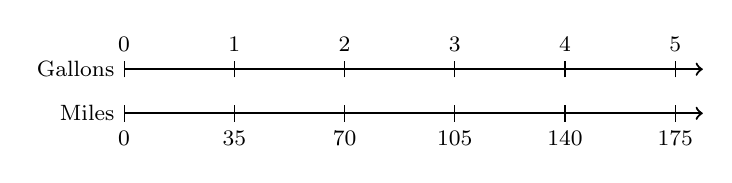
\begin{tikzpicture}[scale=0.7]
  \draw[thick,->] (0,0.8) -- (10.5,0.8);
  \draw[thick,->] (0,0) -- (10.5,0);
  \node[left] at (0,0.8) {\footnotesize Gallons};
  \node[left] at (0,0) {\footnotesize Miles};
  \foreach \x/\g in {0/0, 2/1, 4/2, 6/3, 8/4, 10/5}
  {
    \draw (\x,0.65) -- (\x,0.95);
    \node[above] at (\x,0.95) {\footnotesize $\g$};
  }
  \foreach \x/\m in {0/0, 2/35, 4/70, 6/105, 8/140, 10/175}
  {
    \draw (\x,-0.15) -- (\x,0.15);
    \node[below] at (\x,-0.15) {\footnotesize $\m$};
  }
\end{tikzpicture}
\end{center}
\end{questionText}
\correctAnswer{$245$ miles}
\explanation{From the double number line, $1$ gallon $= 35$ miles. For $7$ gallons: $7 \times 35 = 245$ miles.}
\end{practiceQuestion}

\begin{practiceQuestion}{m-1-6-q30}{gsa}
\begin{questionText}
The table shows the cost of renting a kayak by the hour. Estimate the cost of a $5$-hour rental, then find the exact cost.

\begin{center}
\begin{tabular}{|c|c|}
\hline
\textbf{Hours} & \textbf{Cost} \\
\hline
$1$ & $\$8.50$ \\
\hline
$2$ & $\$17.00$ \\
\hline
$3$ & $\$25.50$ \\
\hline
$4$ & $\$34.00$ \\
\hline
\end{tabular}
\end{center}
\end{questionText}
\correctAnswer{$\$42.50$}
\explanation{Estimate: about $\$9$/hour, so $5 \times 9 \approx \$45$. Exact: $\$8.50 \times 5 = \$42.50$. Check: $\$42.50$ is near $\$45$. \checkmark}
\end{practiceQuestion}
